
The previous chapter introduced the abstract idea of geometric programming with the Geometron Virtual Machine and the Geometron Hypercube.  In this chapter we dive into the specifics of how this is implemented on the Geometron Server so that we can create, edit, and most importantly share symbols from a web browser.  The heart of what is described in this chapter is the Symbol app which exists at symbol.html on every Geometron Server.

In the Symbol app, we can build Geometron glyphs either using a specially marked keyboard or soft keys in a control panel.  To learn the system, it is best to first get a keyboard and mark it up with the symbols so that you can see what you are doing as you learn.  The examples and figures in this section give keyboard values along with symbols in many cases so that you can follow along if the keyboard is not marked and can get used to the layout.  The layout is easy to change, and presumably will evolve over time, but for starting it makes sense to copy whatever keyboard layout the person sharing the system with you uses, in this case me.  See the figure with the keyboard layout for guidance, and go ahead and put markings on keys with these symbols.  I also encourage the further decoration of Geometron Keyboards, with extensive paint and modification so that it retains the distinctive flair of Trash Magic(rainbow paint and googly eyes).   Paint pens are ideal for this, but nail polish or other permanent paints which can be applied with fine lines can all work. A less permanent solution can be found with masking tape on the keys and symbols drawn on the tape.  Stickers can also be printed out and applied to keys.
     
\begin{figure}
	\centering
	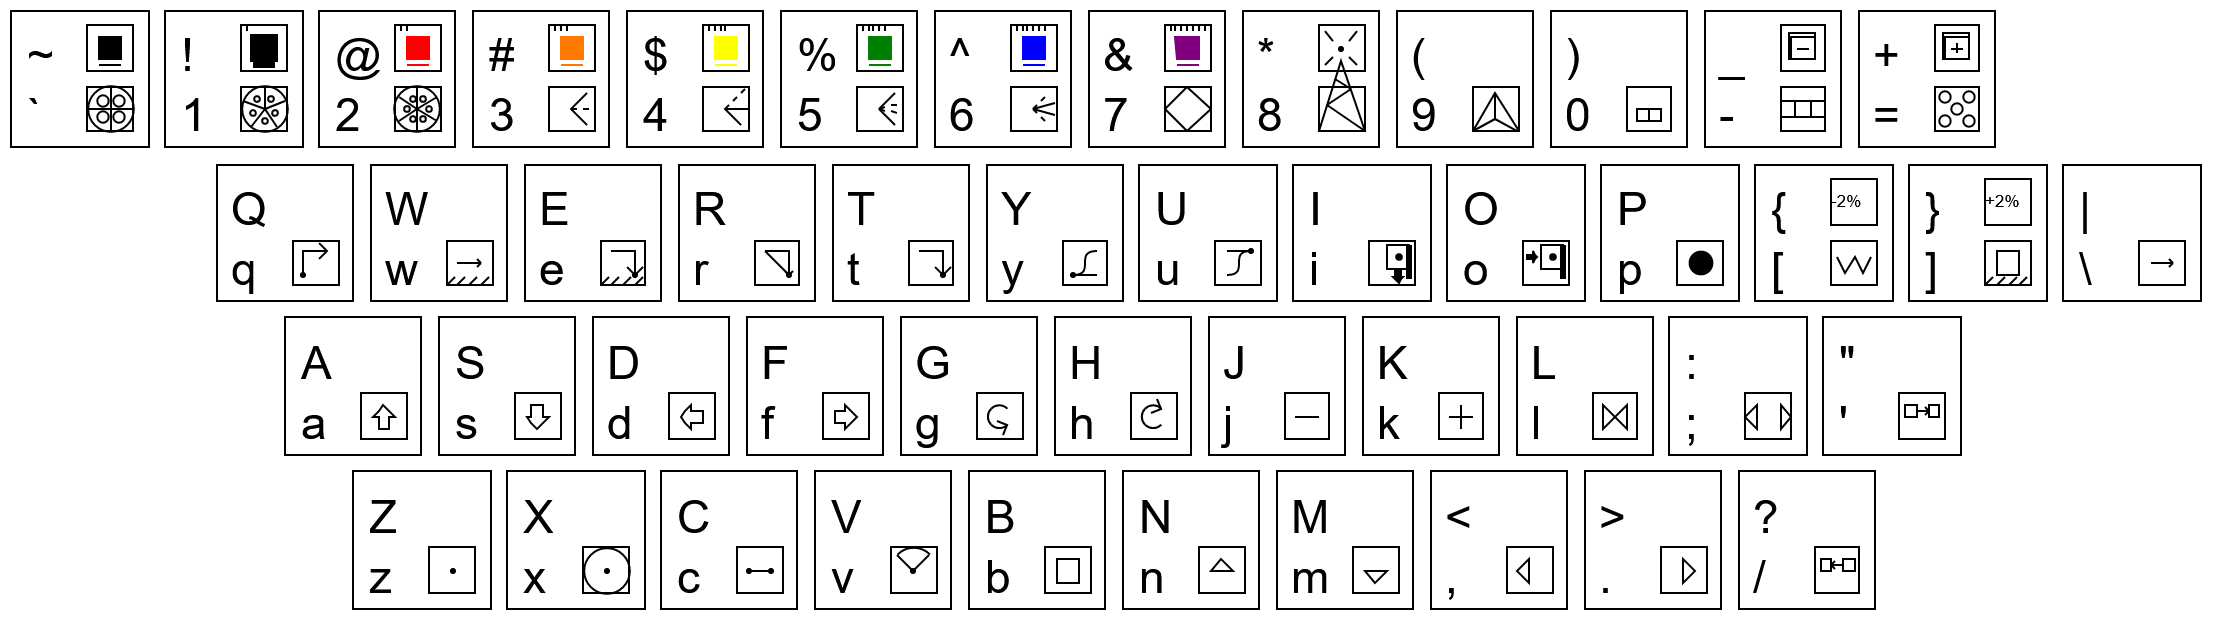
\includegraphics[width=4in]{figures/web2d/keyboard.png}
	\caption[keyboard]
	{Keyboard layout.  Strike a key to add an action to the glyph you are editing.  Arrow keys and backspace allow for editing the whole glyph.  Up and down arrows move to the end or beginning of the glyph.}
\end{figure}

The control panel of soft keys should be pretty self-explanatory: the buttons do the same thing as the keys on the keyboard and are there to make the system work with a touch screen when no physical keyboard is connected, as with smart phones and tablets.

With the ability to edit the main glyph, the best way to learn the language is to just try stuff.  This chapter is largely pictorial.  Go through the figures and try to copy them on the system you are using, play with all the different symmetries, scales, layers, and functions.  To save a symbol, hit the save icon which is in the far left of the menu bar at the top of the screen.  When you have saved a symbol you can see it and download it from the Symbol Feed, which is an icon three in from the left showing equilateral triangles separated by an arrow.  Each symbol is stored as both a bitmap in .png format and a vector graphics file in .svg format.  What is listed in this Feed is simply a sequence of stored files in the directory symbolfeed/, which exists on every Geometron server.  Each file is named with the UNIX timestamp which describes the exact moment it was created.   The Symbol Feed, like all Feeds in the System, also has delete buttons to delete any of the symbols in the Feed, following the Law of Geometron that everything dies.  If you click on an .svg file in the Feed, it will load that symbol into the editor, and you can then go back and edit a copy of it, and save it again to make a modification.  The Symbol Feed also has an upload button just like the Local Image Feed, which lets you upload .svg files from other systems and allow you to edit them using the copy as a template.  Thus we can freely replicate, edit, delete and replicate again.

Move the cursor around, draw circles and lines and squares.  Make polygons, explore scales and symmetries. Try out the Bezier path drawing.  Play with colors.  Make closed and open paths.  When in doubt, destroy it all and start over. 

As you create and edit the main glyph, the address sequence will update live in the text field next to the one where the cursor is for editing.  This will be a sequence of numbers all of which begin with 0.  As with all other parts of the Geometron system, the ability to share information instantly across the world with it is of the highest importance. If you copy the sequence of addresses in that field to the clip board and send it via text message, email or pastebin to someone else with Geometron, they can paste it in that same field and hit return and they will instantly load the same glyph you created, which they can then edit and send back to you modified.  

What you are editing in the system is not just a glyph but a whole JSON structure which is how we can share a whole symbol including style, position, scale, and custom symbolic language tools.  This structure will be described in more detail below, but you can immediately start sharing them by clicking on the icon which says JSON in the Symbol app.  This will bring up a screen which has the JSON data in a text area, and a set of buttons to export, import, save, or reset.  Reset is important because it is possible to corrupt the data beyond recognition and this gets you back to something which will definitely work.  As with all other components of the Geometron system, this is a human readable text format which is designed to be shared both by direct text messaging and by copy and pasting into public pastebins and sharing the pastebin link.



\begin{figure}
	\centering
	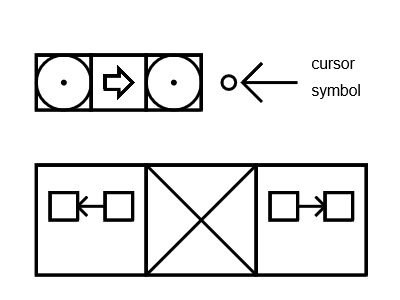
\includegraphics[width=3in]{figures/web2d/cursoredit.png}
	\caption[cursoredit]
	{Edit symbols.  This shows the symbols for moving the cursor back and forward, deleting an action, and also shows what the cursor looks like in a glyph being edited.}
\end{figure}


\begin{figure}
	\centering
	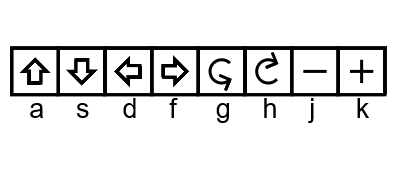
\includegraphics[width=4in]{figures/web2d/move.png}
	\caption[move]
	{Movements.  Arrows move along directions of the lines in the cursor.  Rotation is by the unit indicated by the cursor wing angles. Scale actions are by the current scale value as shown by the dot positions on the cursor.  Letters shown indicate the keys which map to these actions on a QWERTY keyboard with the default settings.}
\end{figure}

\begin{figure}
	\centering
	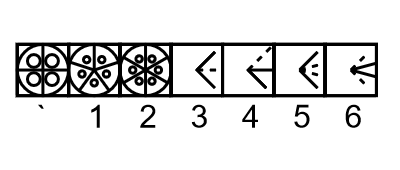
\includegraphics[width=4in]{figures/web2d/angles.png}
	\caption[angles]
	{Angles described by symmetry glyphs.  This also shows the actions to bisect, double, trisect and triple angles, and what keys are used to activate each geometric action.}
\end{figure}

\begin{figure}
	\centering
	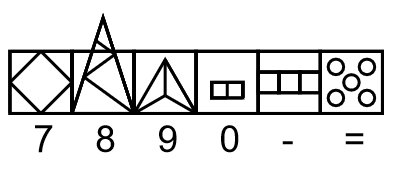
\includegraphics[width=4in]{figures/web2d/scaleactions.png}
	\caption[scaleactions]
	{Scales, along with keys used to map to them in default configuration. There is no relation between the numbers on the keys and the mathematics of the scales.  The scales shown are, from left to right, the square root of 2, the Golden Ratio, the square root of 3, 2, 3, and 5.}
\end{figure}

\begin{figure}
	\centering
	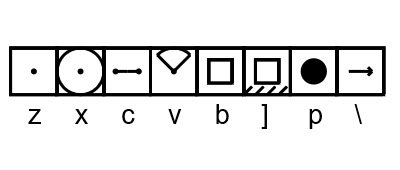
\includegraphics[width=4in]{figures/web2d/basicdraw.png}
	\caption[basicdraw]
	{Basic drawing actions, along with keys used in default configuration to activate them.  From left to right the actions are: draw dot, draw circle of unit radius, draw line segment of unit length, draw arc between cursor wings, draw a square, draw a filled square, draw a filled circle, and draw a line segment while moving forward one unit.}
\end{figure}

\begin{figure}
	\centering
	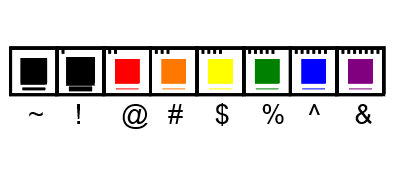
\includegraphics[width=4in]{figures/web2d/colors.png}
	\caption[colors]
	{Layers. Each layer has a line color, line width, and fill color, all of which are set with the Style object using the Style editor app.}
\end{figure}


\begin{figure}
	\centering
	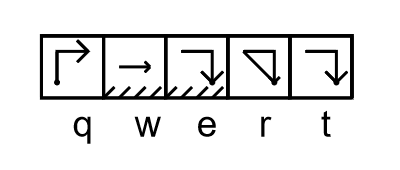
\includegraphics[width=4in]{figures/web2d/pathactions.png}
	\caption[pathactions]
	{Path actions, with keys used to activate them in default state.  From left to right, actions are: start path, draw line segment in path, close a filled path, close an unfilled path, and terminate a path without closing it.}
\end{figure}

\begin{figure}
	\centering
	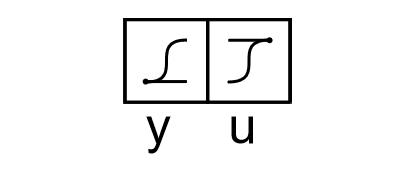
\includegraphics[width=4in]{figures/web2d/bezieractions.png}
	\caption[bezieractions]
	{Start a Bezier Path and terminate it with the y and u keys.}
\end{figure}


\begin{figure}
	\centering
	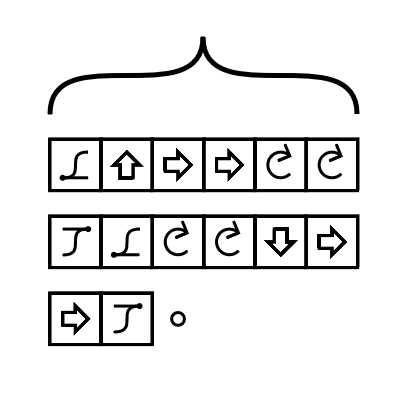
\includegraphics[width=4in]{figures/web2d/bezierbracket.png}
	\caption[bezierbracket]
	{Demonstrating the power of Geometron to make useful symbols with Bezier paths quickly and easily: a twiddle bracket.}
\end{figure}


\begin{figure}
	\centering
	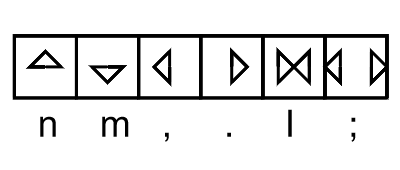
\includegraphics[width=4in]{figures/web2d/panzoom.png}
	\caption[panzoom]
	{Pan and zoom the field of view.}
\end{figure}

\begin{figure}
	\centering
	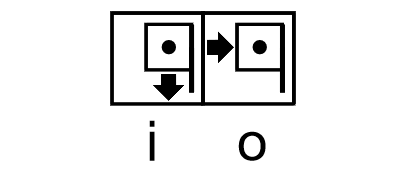
\includegraphics[width=4in]{figures/web2d/flagactions.png}
	\caption[flagactions]
	{Drop a flag, return to flag.  This saves and then recalls the state of the GVM.}
\end{figure}


\begin{figure}
	\centering
	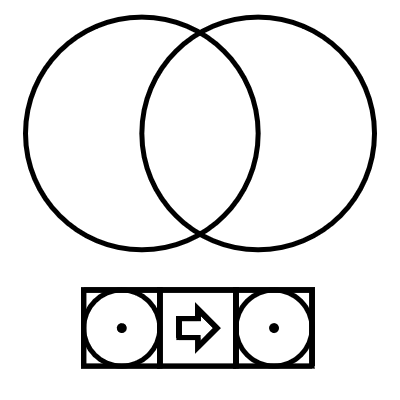
\includegraphics[width=4in]{figures/web2d/vesicapiscis.png}
	\caption[vesicapiscis]
	{The ``hello world'' of geometric programming, the Vesica Piscis.}
\end{figure}
\begin{figure}
	\centering
	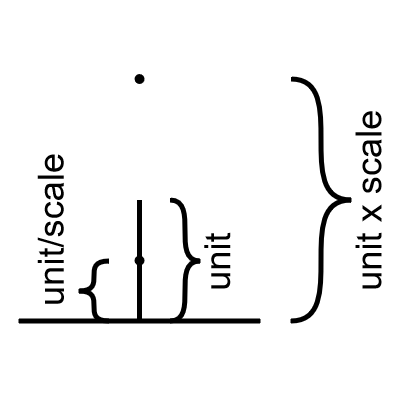
\includegraphics[width=4in]{figures/web2d/cursorscale1.png}
	\caption[cursorscale]
	{Cursor scale.  This shows how scale works with the Geometron cursor.}
\end{figure}
\begin{figure}
	\centering
	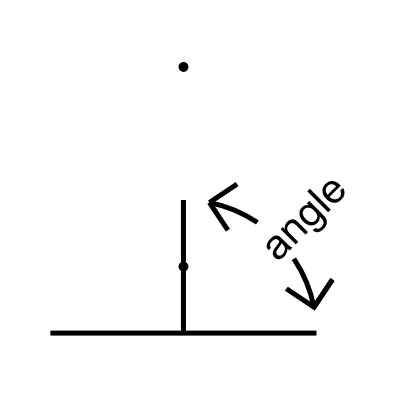
\includegraphics[width=4in]{figures/web2d/cursorangle1.png}
	\caption[cursorangle]
	{Cursor angle. This shows how angles work with the Geometron cursor.}
\end{figure}
\begin{figure}
	\centering
	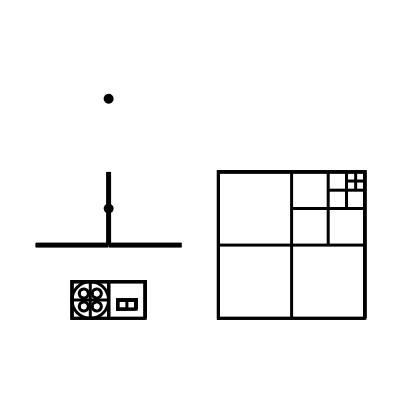
\includegraphics[width=4in]{figures/web2d/cursorsquare.png}
	\caption[cursorsquare]
	{What the cursor looks like with factor of two scaling and a 90 degree angle.  Also shown is a square used in Action Geometry.  Try making the square!}
\end{figure}
\begin{figure}
	\centering
	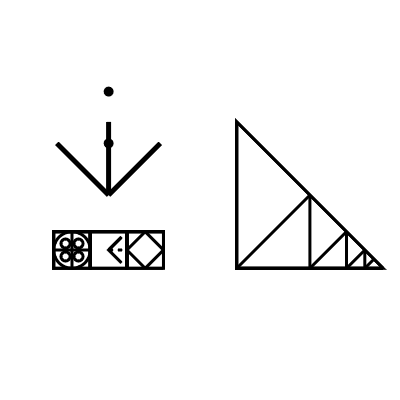
\includegraphics[width=4in]{figures/web2d/cursorroot2.png}
	\caption[cursorroot2]
	{Another example of a commonly used Geometron cursor state, which combines the square root of two with 45 degree angles.  Also shown is yet another shape used in Action Geometry which is also a good exercise to try to copy yourself.}
\end{figure}
\begin{figure}
	\centering
	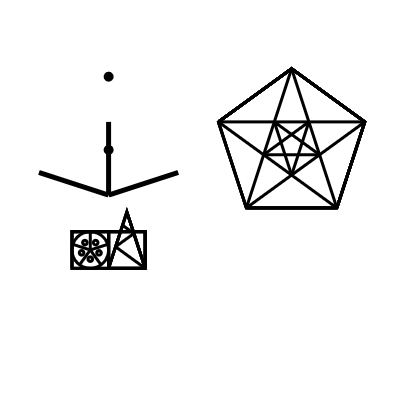
\includegraphics[width=4in]{figures/web2d/cursorgolden.png}
	\caption[cursorgolden]
	{Cursor with Golden Ratio scaling and 72 degree angle for fivefold symmetry work.  Shown is another shape that is helpful to learn to copy, the pentagon/pentagram fractal.}
\end{figure}
\begin{figure}
	\centering
	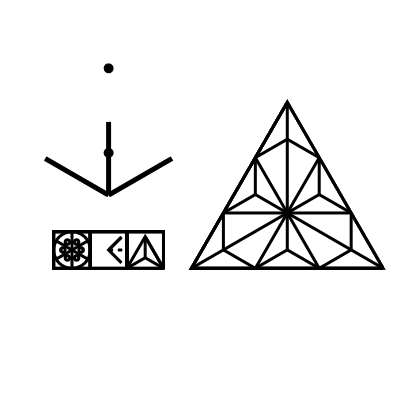
\includegraphics[width=4in]{figures/web2d/cursorroot3.png}
	\caption[cursorroot3]
	{Cursor with square root of three scaling and 60 degree angle.  This can be used to make the kinds of symbols shown, and replicating that is a useful exercise, as well as working through the deconstruction of the six pointed star and hexagon.}
\end{figure}
\begin{figure}
	\centering
	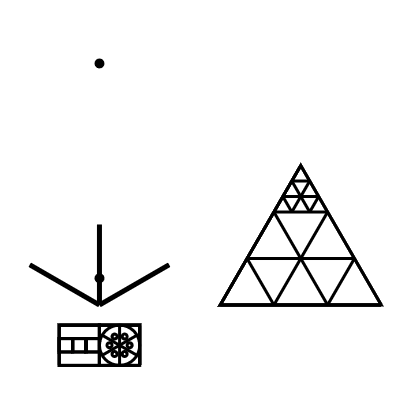
\includegraphics[width=4in]{figures/web2d/cursor3.png}
	\caption[cursor3]
	{The cursor with a 60 degree angle and factor of 3 scaling, along with another exercise to copy.}
\end{figure}
\begin{figure}
	\centering
	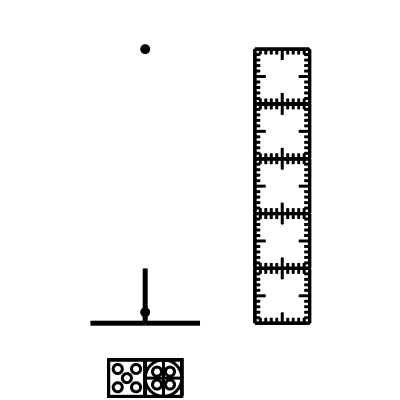
\includegraphics[width=4in]{figures/web2d/cursor5.png}
	\caption[cursor5]
	{Cursor with scaling factor 5 and right angles. This can be used along with scale factor 2 to make things with scale factor 10.  What is shown to copy as an exercise is a ruler constructed using this tool which can be made physical using a laser cutter as discussed in the Action Geometry chapter.}
\end{figure}


Each instance of the Geometron Virtual Machine has a style object, which defines 8 layers, numbered from 0 to 7.  Each style has a line color, line width, and fill color.  The properties of the style object are stored in the JSON file data/currentjson.txt which is used by the app symbol.html to edit graphics which are used by the rest of the Geometron system.  

\begin{figure}
	\centering
	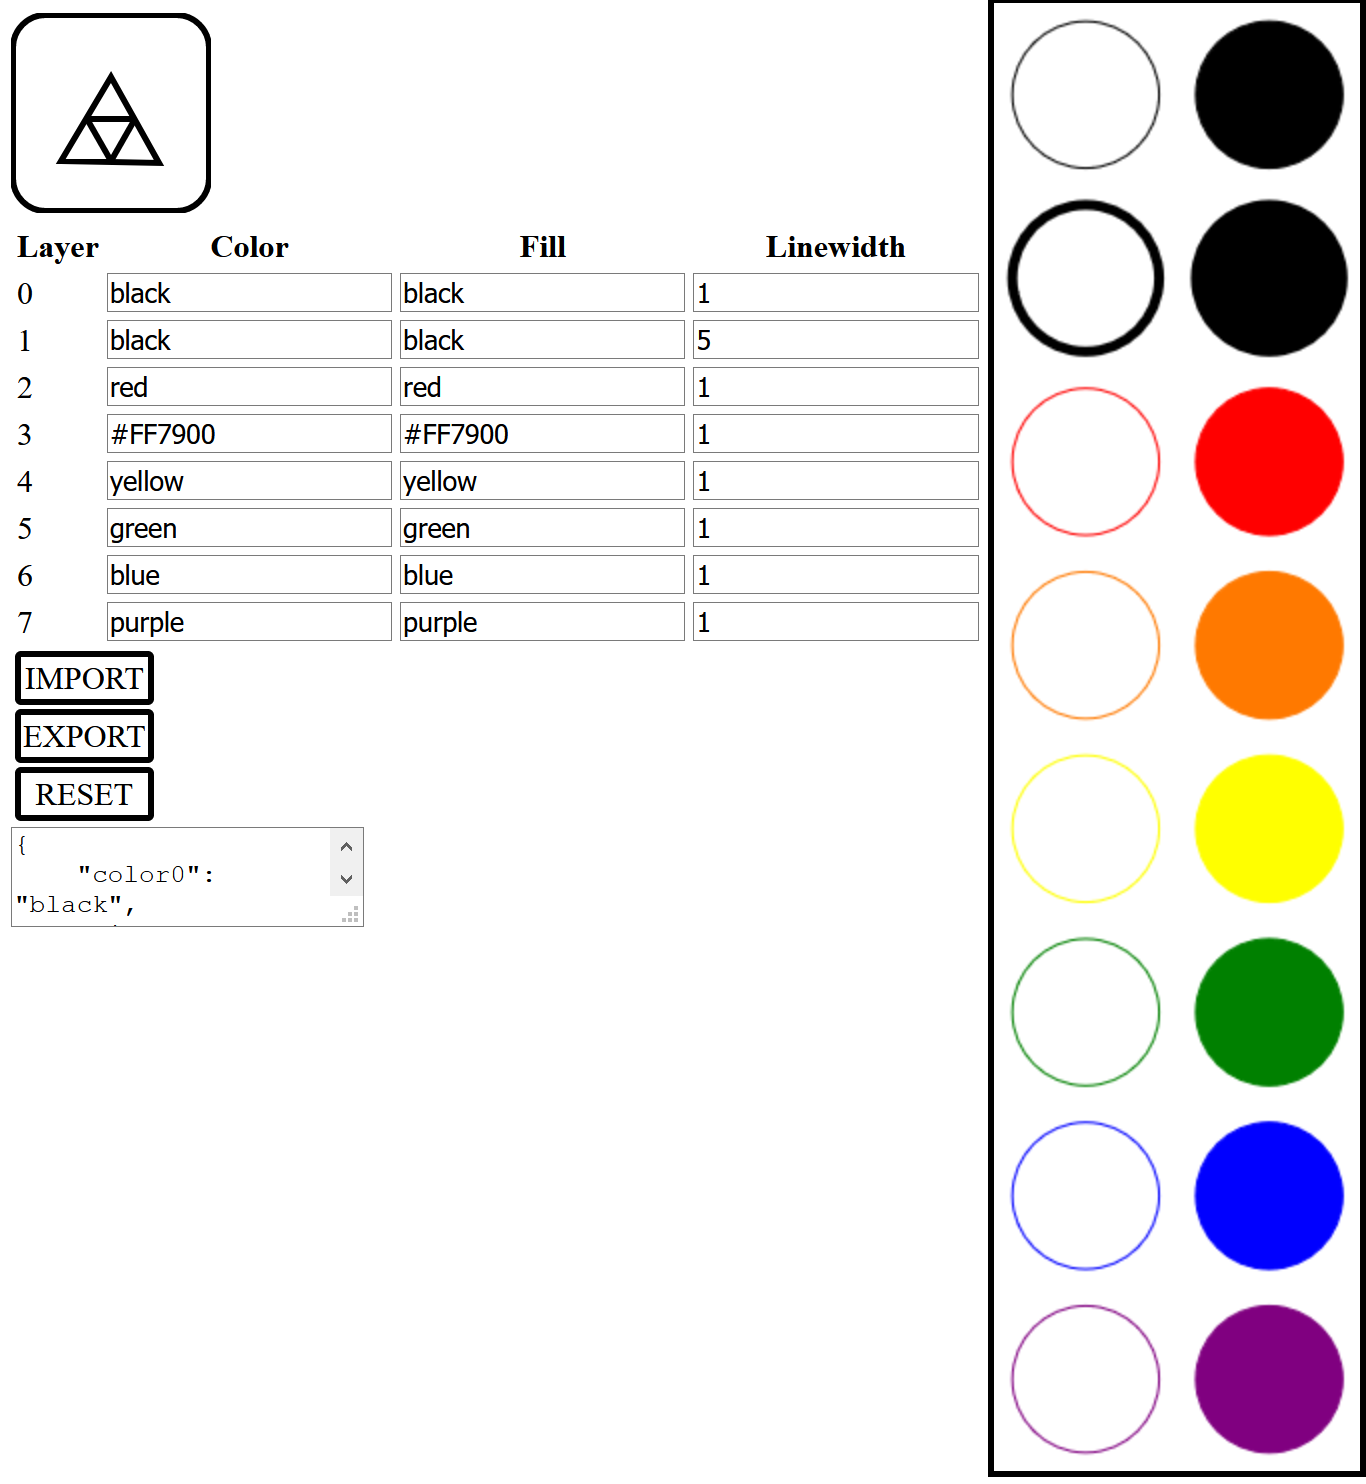
\includegraphics[width=4in]{figures/web2d/styleeditor.png}
	\caption[styleeditor]
	{Screen shot of the style editor app at styleeditor.html.  The display on the right hand side of the screen shows an unfilled circle and filled circle of each layer's style.  The text area in the bottom left of the screen is used to import and export style data, which can be saved offline and shared with other users via text message, email, etc.  The RESET button resets the style to a standard setting, which will erase any changes made to the existing style. Enter new values into any field to immediately change it.}
\end{figure}

While the style app edits the data file currentjson.txt which applies to the whole Geometron object used for symbol editing, the importing and exporting of data for sharing with other users only includes style information, without the rest of the JSON data.  This allows styles to be separated from the rest of the information for the purposes as usual of building a robust remix culture where Geometron users can constantly be sharing each piece of the system.  The EXPORT button will always post the current style JSON in the window in the lower left of the screen.  IMPORT will import the data, and RESET returns it to a default state.  Try creating your own new style with unusual line widths and colors, then exporting it and saving it offline, sharing it with other users, etc.  

Colors are in the format of HTML/CSS/JavaScript, and can be either names of colors like ``red'' or RGB color values like ``\#00ff00''.  This last format is a number in base 16 which has three 2 digit numbers in it(numbers between 0 and 0xFF), where the three numbers are values of red, green, and then blue.  So black is \#000000 and white is \#FFFFFF.  Any value where all three numbers are the same, like \#808080 will be a shade of grey.   Colors can be partially transparent by adding a fourth hexidecimal number which represents opacity.  So fully opaque red is \#FF0000FF, and red with half transparency is #FF000080(80 because 8 is half of 16, this is actually 128 in decimal).

The next section of the JSON we want to know how to edit in order to be able to make useful graphics is the setup, edited in the app setup.html.  Setup edits five numbers, all of which are in units of pixels: x0, y0, unit, width and height.  Width and height are the width and height of the graphics file currently being edited or created.  When a Geometron glyph is drawn with a given GVM, it starts with x and y equal to x0 and y0. Setting these two values is therefore effectively setting the horizontal and vertical offset of the field of view of the symbol.  When we activate a pan function within the symbol.html app what we are really doing is modifying the values of x0 and y0 in the JSON file.  These are done manually in this app.  Finally, unit describes the initial unit value of the GVM.  This is essentially the scale factor.  So again when we activate the zoom functions in any other symbol editor what we are really doing is making changes to the variable unit in the global JSON file.    

The app setup.html has five fields in which to enter the numbers for the five values. There is also a reset button to restore default, with a 600 by 600 pixel square and 80 pixel unit centered in the center.  

The final section of the global JSON file which defines the settings of the symbol app is the shape stack.  This is a subset of the hypercube, and is stored both in the JSON file data/hypercube.txt and also data/currentjson.txt.  When vector graphics files are saved, this shape stack is stored inside them so that they can be reloaded with the whole stack.  The creating and sharing of useful shape stacks will be discussed in the next chapter.  This is a very important element of the system as it allows for the rapid dissemination of specialized graphical languages for things like drawing circuit diagrams or subway maps.

Other links to other apps from the main symbol app are to the keyboard editor, which edits the layout of the keyboard, the Hypercube editor, which edits the entire Geometron Hypercube, and the Font editor, which edits just the font.  All these have the capacity to share human readable text from system to system as is the case with everything in the Geometron system.  The font and Hypercube apps are still somewhat crude and could be improved substantially, but they do work for their intended purpose with a little bit of fiddling.  They will be used through the rest of this work as we delve into more applications of Geometron geometric programming. 

There is also an app separate from the main symbol editor called symboltrace.html, which allows you to trace images into symbols, which you can then copy and paste at will.  This takes images from both the local and global image feed, so you will need to load the image you want to copy in one of those first.  Still another random app of some utility is action2symbol.html, which converts a glyph made up of actions to one made up of the symbols which correspond to those actions.  This is how we put glyph symbol spelling into a symbol, which is very useful for documenting things which reference the language and how it is used.  

Part of the power of the Symbols in Geometron is how they are integrated into the rest of the system.  When you save a symbol, a copy of the base 64 encoded bitmap is stored in the textfeed which gets used by the Map editor to create maps.  This means that you can create a symbol, then go import it into the Map editor immediately.  Because it is a self-contained image url which has the actual graphics encoded in the url rather than as an external file, this Map you create can then be shared with anyone else anywhere in the world with another Geometron system and they will be able to import and use that Map without any other image files.  This ability to instantly integrate Symbols into Maps can enable a sort of graphical meme system which can be extremely powerful for numerous applications.


Also, we note that all icons used in the Geometron system are created using the Symbol editor described in this section.  These are then stored in the directory iconsymbols/.  This directory is all copied with every copy of the whole self-replicating system.  Therefore if you want to add another symbol to the next copy of the system, just add your new symbol to this directory, run dnagenerator.php, and the next instance will have your new image.

If you are a coder, you can read the whole of the system documented in this chapter in the JavaScript library stored at jscode/geometron.js, which is on every instance of the system.  You can of course edit this, and your edits will replicate along to the next instance of the system.
